\section{Background}



\noindent\textbf{ReAct Paradigm for Agents.}
Most modern agentic workloads follow the ReAct paradigm~\cite{react}, in which an LLM repeatedly alternates between reasoning over accumulated context and invoking external tools.
In contrast to single-turn inference, this execution model induces long-horizon, multi-turn workflows where intermediate thoughts, tool outputs, and observations are continuously appended to the prompt across dozens or even hundreds of steps~\cite{aflow,gptswarm,sppo}.


Consequently, an agent’s context and its associated KV cache footprint evolve monotonically over the agent’s lifetime as shown in Figure \ref{fig:comparisons}.
This unbounded, step-dependent growth fundamentally alters the memory and execution semantics of LLM inference, turning KV cache from a short-lived optimization into a long-lived, shared system resource.
% Existing LLM serving designs, which are optimized for short and independent requests with fixed prefixes, fail to account for this shift.


\noindent\textbf{Prefix Caching in LLM Serving Engines.}
To facilitate fine-grained prefix reuse and eliminate redundant computation, modern LLM serving engines \cite{sglang,pagedattention} organize the KV cache into a tree structure on the GPU, to make full use of shared prefixes and reduce memory usage.  
Each node in the tree stores a contiguous segment of tokens and its corresponding KV cache slots.
Upon receiving a new request, the system matches the prefix from the root of the tree and concatenates the KV cache slots along the matched path to reconstruct the cached prefix.
When GPU memory becomes insufficient, cache nodes are evicted based on a Least Recently Used (LRU) policy.


These designs are effective for workloads composed of short, independent requests with stable prefix reuse.
However, under agentic batch inference, KV cache demand is both long-lived and highly dynamic, while eviction decisions remain purely recency-based. See \S\ref{sec:motivation} for detailed analysis.
% As a result, cache entries that are semantically critical to an agent’s progress can be evicted during periods of inactivity, even when the total number of agents is fixed.
% Figure~\ref{fig:twoagent} illustrates how this mismatch leads to persistent memory pressure and unstable cache behavior as execution progresses.

To alleviate GPU memory pressure, many systems introduce CPU memory as a secondary cache layer and offload evicted KV cache slots over PCIe.
Although offloading is often faster than recomputation in isolation~\cite{Ragcache,CachedAttention,mooncake,sppo,internevo}, its effectiveness degrades under high concurrency.
Simultaneous offload and reload operations contend for PCIe bandwidth and incur additional synchronization overheads, causing per-step latency to increase sharply as shown in Figure \ref{fig:comparisons}c.
This limitation suggests that KV cache management strategies optimized for low-concurrency or request-centric workloads may perform poorly in agentic batch inference.


\begin{figure}[tb]
    \centering
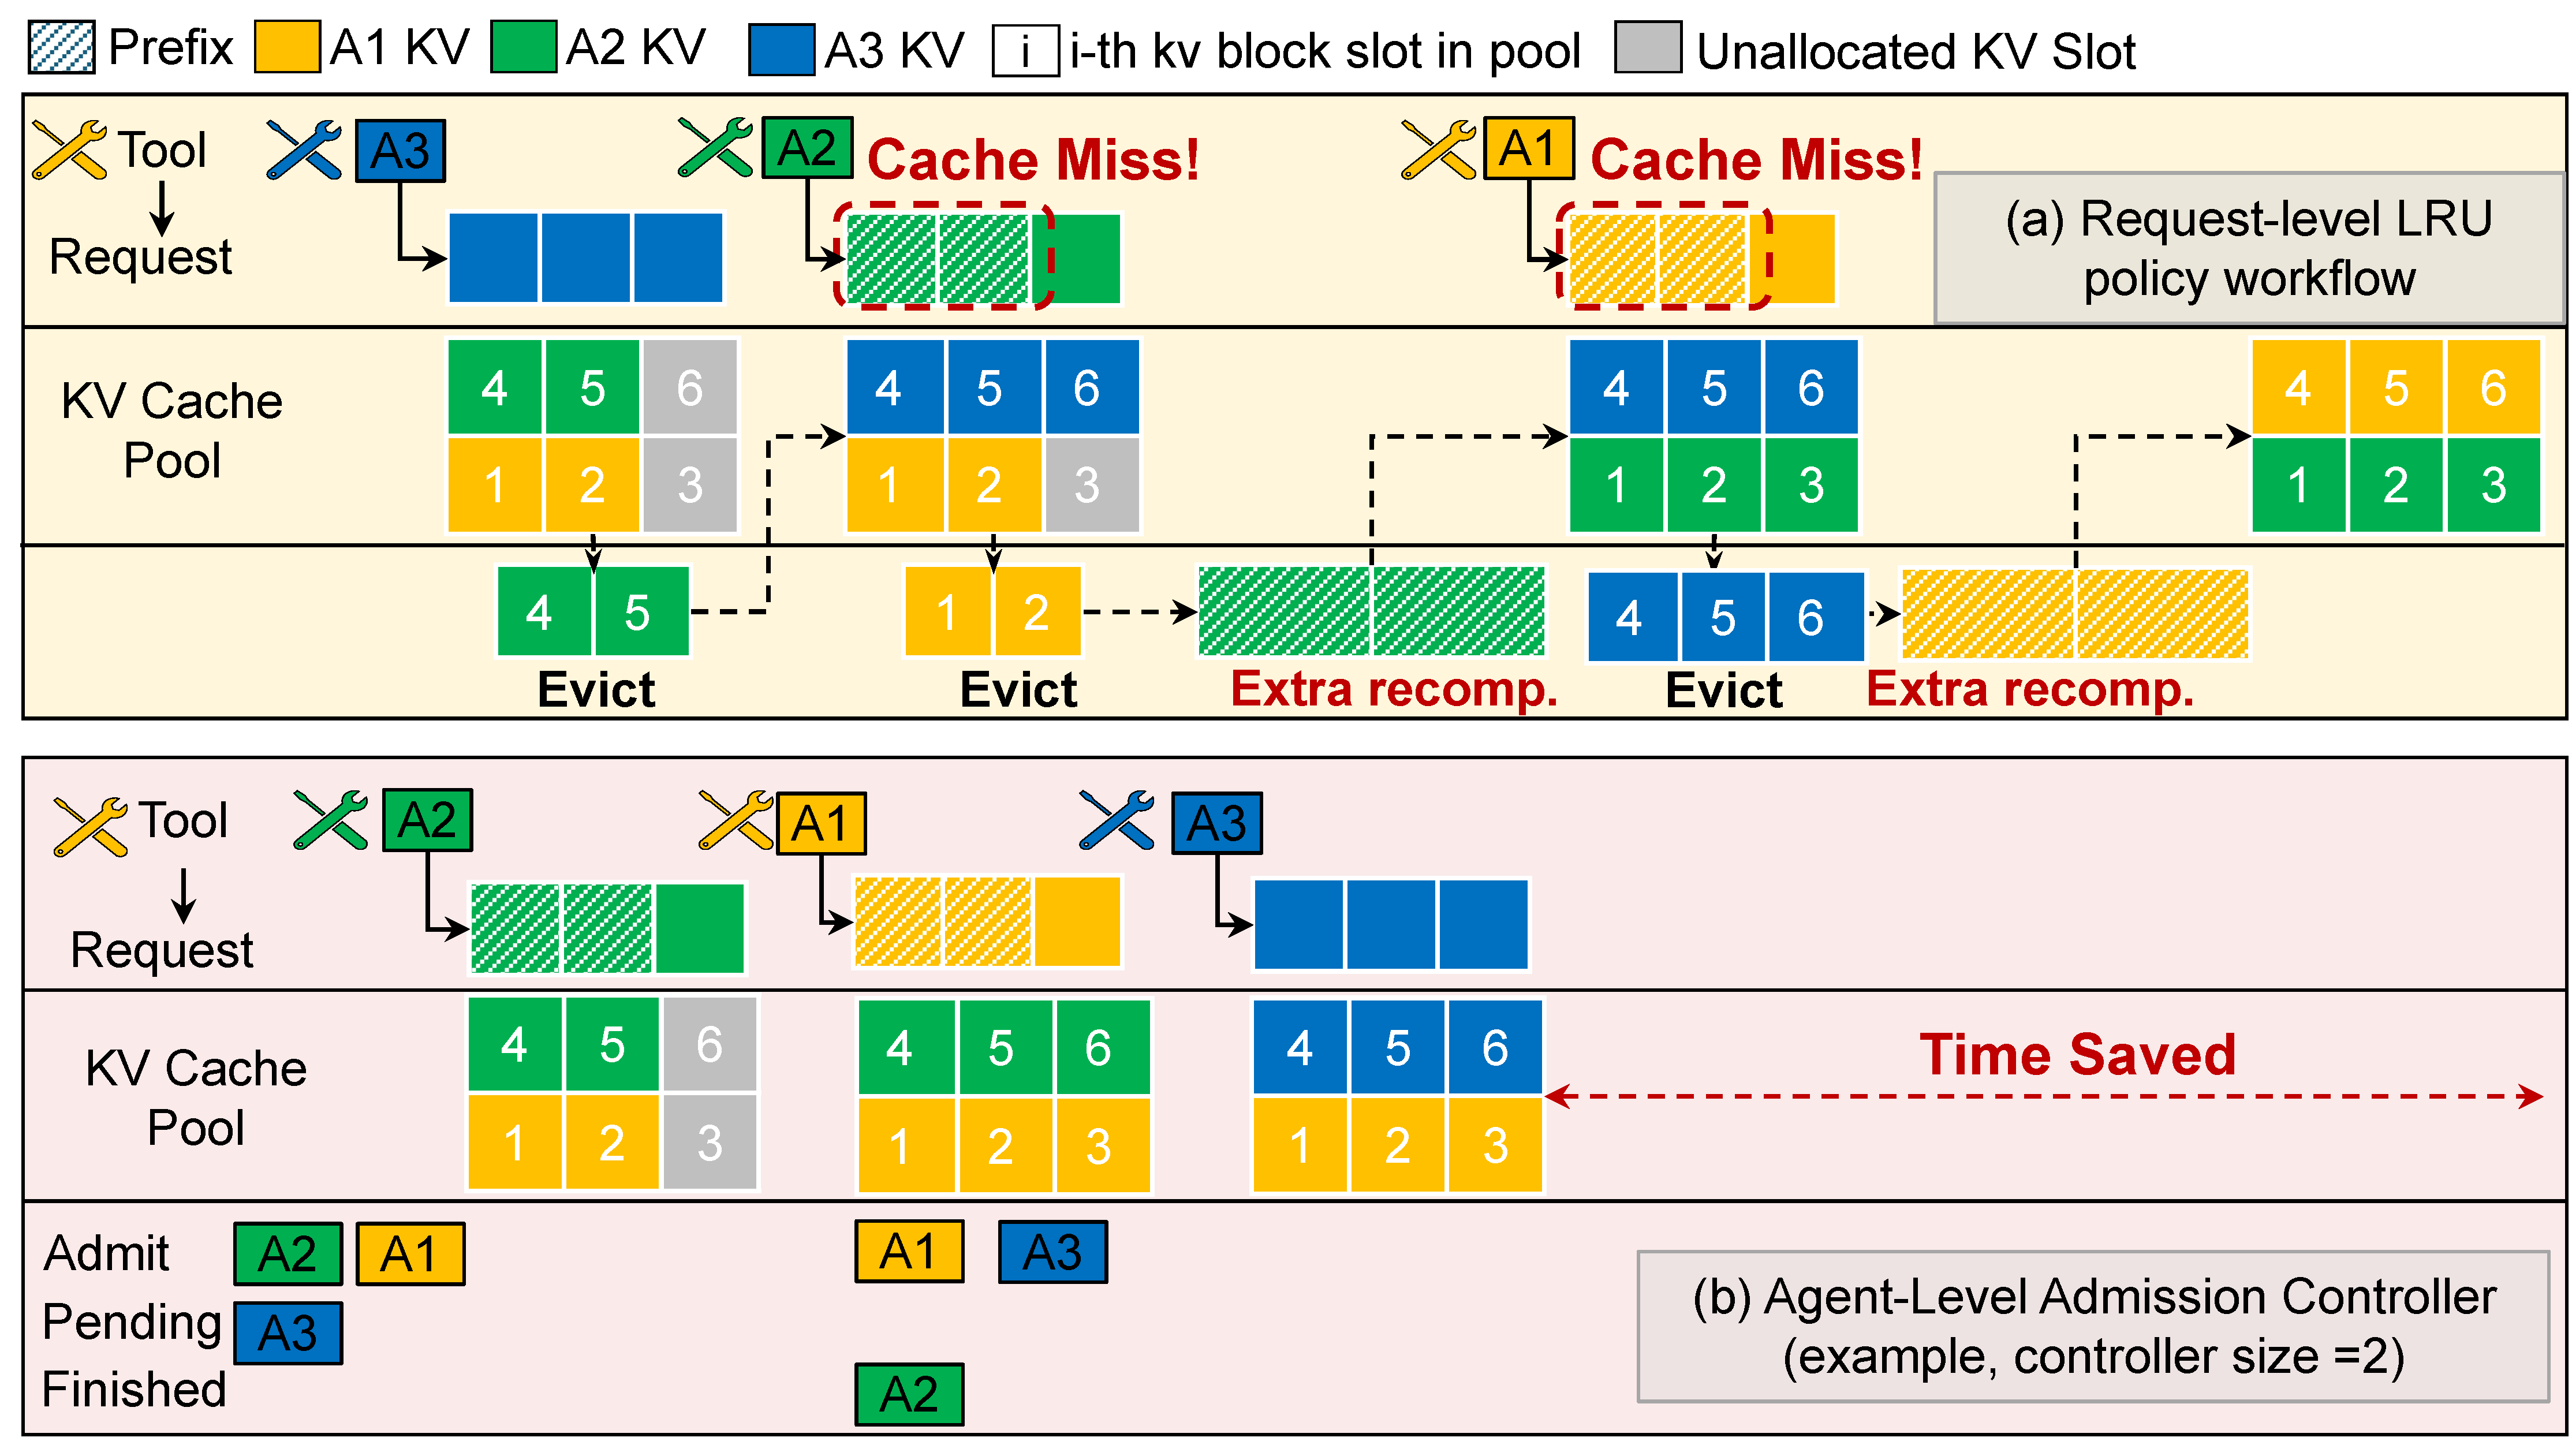
\includegraphics[width=0.98\linewidth]{figure/3agents.pdf}
    \caption{Three-agent workflow illustrating middle-phase thrashing and agent-level admission control. (a) LRU eviction causes paused agents to lose KV cache entries, triggering repeated recomputation and middle-phase thrashing. (b) Agent-level admission control bounds concurrency, preventing cache overcommitment and eviction-induced recomputation.}
    \label{fig:twoagent}
    % \vvspace{}
\end{figure}





% Memory exhaustion can arise for two primary reasons.
% The first is a high degree of concurrency, where many requests execute distinct agentic workflows simultaneously, leading to a large number of active KV cache entries.
% The second, which is particularly relevant to agent-based workloads, is the continual growth of prefix length as an agent executes multiple reasoning or interaction rounds.
% Unlike single-turn prompts with a fixed prefix, agent execution repeatedly appends intermediate observations, tool outputs, and generated responses to the context, as shown in Figure \ref{fig:comparisons} (a), the input length increasing across 10 agent reasoning steps.
% As a result, the KV cache footprint of a \emph{single agent} increases monotonically with the number of agent steps as shown in Figure \ref{fig:comparisons} (b), significantly amplifying memory pressure at longer contexts even under moderate concurrency.

% To mitigate GPU memory pressure, many systems configure CPU memory as a secondary cache layer, allowing evicted KV tensors to be swapped over PCIe.
% Although PCIe access incurs additional latency, prior work has shown that KV cache offloading is generally faster than recomputing the corresponding KV tensors from scratch \cite{Ragcache,CachedAttention,mooncake}.
% Figure \ref{fig:comparisons} (c) compares the PCIe transfer time with the prefill computation time, demonstrating that offloading can be an efficient strategy when memory pressure is low or concurrency is limited.

% However, under high concurrency, PCIe-based offloading can become a performance bottleneck.
% As multiple requests concurrently swap KV tensors, PCIe bandwidth contention and queueing delays can significantly inflate per-step latency, diminishing the advantage of offloading over recomputation.
% Moreover, frequent offload and reload operations introduce additional synchronization and scheduling overheads, which are not captured by isolated offline profiling.
% This observation suggests that KV cache management policies optimized for low-concurrency settings may perform poorly in agentic batch inference.



\noindent\textbf{Congestion Control and AIMD.}
Congestion control has long been studied as a principled mechanism for regulating access to shared and finite resources in distributed systems~\cite{congestion_control}.
In packet-switched networks, multiple senders compete for limited link bandwidth, and uncoordinated transmission can lead to congestion collapse.
To address this, TCP congestion control dynamically adjusts the sending rate based on feedback signals that indicate congestion, such as packet loss or increasing round-trip time.

A widely adopted approach is the Additive Increase Multiplicative Decrease (AIMD) algorithm \cite{chiu1989analysis, AIMD1}:
a sender cautiously increases its congestion window \cwnd\footnote{\cwnd is a sender-side limit that regulates how much data can be sent at once to prevent overwhelming the network.} by a small additive factor when no congestion is observed, probing for additional available capacity.
When congestion is detected, \cwnd is reduced multiplicatively, rapidly relieving pressure on the shared resource.
% Classic TCP variants such as TCP Reno employ AIMD with fixed parameters, increasing cwnd linearly and halving it upon packet loss~\cite{tcp}.
Due to its simplicity and effectiveness, AIMD is widely adopted in many systems, including networking, datacenter scheduling, and distributed storage~\cite{tcp}.
% Beyond networking, AIMD represents a general control principle for achieving stability and high utilization under uncertain and time-varying resource availability.
% By combining gradual exploration with decisive backoff, AIMD enables multiple independent actors to share a constrained resource efficiently without explicit coordination.
% This control paradigm has since inspired resource management designs in diverse domains, including datacenter scheduling and distributed storage systems.

This work draws an analogy between network bandwidth and GPU-resident KV cache capacity during agentic batch inference.
Similar to network links, KV cache is a shared, finite resource whose overcommitment leads to congestion in the form of degraded efficiency, memory fragmentation, and increased execution latency.
Unlike packet networks, LLM inference systems exhibit indirect and delayed congestion signals, as resource usage evolves at the granularity of agent execution rather than individual tokens.
These differences motivate the need to reinterpret congestion control principles (e.g., AIMD) at the agent level to regulate admission and maintain high throughput in agentic batch inference.

